\documentclass[a4,center,fleqn]{NAR}

% Enter dates of publication
\copyrightyear{2008}
\pubdate{31 July 2009}
\pubyear{2009}
\jvolume{37}
\jissue{12}

%\articlesubtype{This is the article type (optional)}

\begin{document}

\title{\textit{dpcR} a Swiss-army knife for the analysis of digital PCR experiments}

\author{%
Micha\l{} Burdukiewicz\,$^{1,6}$,
Jim Huggett\,$^{2}$,
Alexandra Whale\,$^{2}$,
Bart K.M. Jacobs\,$^{3}$,
Lieven Clement\,$^{3}$,
Piotr Sobczyk\,$^{1}$,
Andrej-Nikolai Spiess\,$^{4}$,
Val\'{e}rie Taly\,$^{5}$,
Peter Schierack\,$^{6}$,
Stefan R\"odiger\,$^{6}$\footnote{To whom correspondence should be addressed.
Tel: +49 357385936; Fax: +49 357385801; Email: stefan.roediger@b-tu.de}}

\address{%
$^{1}$Department of Genomics, Faculty of Biotechnology, University of Wroc\l{}aw, Wroc\l{}aw, Poland
and
$^{2}$Molecular and Cell Biology Team, LGC, Teddington, United Kingdom
and
$^{3}$Department of Applied Mathematics, Computer Science and Statistics, Ghent University, Belgium
and
$^{4}$University Medical Center Hamburg-Eppendorf, Hamburg, Germany
and
$^{5}$Universit\'{e} Paris Sorbonne Cit\'{e}, Paris, France
and
$^{6}$Faculty of Natural Sciences, Brandenburg University of Technology Cottbus--Senftenberg, Gro\ss{}enhainer Str. 57, 01968, Senftenberg, Germany
}
% Affiliation must include:
% Department name, institution name, full road and district address,
% state, Zip or postal code, country

\history{%
Received January 1, 2009;
Revised February 1, 2009;
Accepted March 1, 2009}

\maketitle

\begin{abstract}

The digital Polymerase Chain Reaction (dPCR) enables an absolute 
quantification of nucleic acids. Different statistical analysis frameworks
were proposed. However, most analysis is done in closed source software as 
provided by the vendors. This makes it harder to compare results, such as the 
confidence interval estimates. An unified open software framework for 
reproducible research is not available.

To perform dPCR analysis we implemented peer-review statistical methods and 
plots into the \textit{dpcR} framework, based on the sophisticated statistical 
computing environment \textbf{R}. \textit{dpcR} is versatile open source 
cross-platform software framework, which provides functions to process dPCR data 
independent of the hardware. Our software can be used for data analysis and 
presentation, as framework for novel technical developments and as reference for 
statistical methods in dPCR analysis. Features such as functions to estimate the 
underlying Poisson process, calculation of confidence intervals based on single 
samples as well as on replicates, a novel Generalized Linear Model-based 
procedure to compare digital PCR experiments and a spatial randomness test for 
assessing plate effects have been integrated. We use a plug-in like architecture 
and abstraction layers to make the framework usable for droplets and (real-time) 
chamber based technologies.

\textit{dpcR} is implemented with interfaces to the command-line, graphical 
user interfaces and interactive web application. Therefore, it can be used by 
novices in a graphical user interface or by experts via a command-line 
interface. The \textit{dpcR} framework can be used to build a custom-made 
analyser according to the user requirements. \textit{dpcR} is an 
open framework, which can be easily adapted to the growing knowledge in dPCR. 

\end{abstract}


\section{Introduction}

The digital PCR (dPCR) is an important contender for precise nucleic acids 
quantifications. Application of the dPCR include investigation of allele 
frequencies, gene expression analysis and absolute quantification of PCR 
products. The chemical basis (e.g., buffer, primer) of the dPCR and thermal 
cycling is similar to the real-time quantitative qPCR (qPCR). Though, approaches 
based on isothermal amplification were also developed 
\cite{pabinger_survey_2014, rodiger_r_2015}. A first proposal for a dPCR like 
approach and the use of the Poisson distribution to quantify the number of 
molecules on a ``sample'' was shown by Ruano \textit{et al.} 1990 (PNAS) with 
the single molecule dilution (SMD) PCR \cite{ruano_haplotype_1990}. In 1999 
Vogelstein \textit{et al.} (PNAS) described the first true digital PCR 
\cite{vogelstein_digital_1999}. In contrast to qPCR, the amplification reaction 
does not take place in a single reaction chamber. Rather its a process of clonal 
amplification in small separate ``partitions'' (e.g., nl volume droplets of 
water oil emulsions, chambers on micro structured chips). The number of positive 
partition in relation to the number of total partitions. By applying Poisson 
statistics it is possible to determine the number of the starting material in 
given volume. Therefore, the dPCR does not require an external calibration 
\cite{selck_increased_2013, rodiger_r_2015}. Since approximately ten years the 
digital PCR (dPCR) is gaining momentum in the mainstream user-base and will 
likely have the same impact as the qPCR methodology \cite{huggett_qpcr_2015, 
morley_digital_2014, rodiger_r_2015}. There is an intensive research on dPCR 
platforms with the overall aim to make to technology broadly usable, cheap, 
robust and to enable high sample throughput.

% **************************************************************
% Keep this command to avoid text of first page running into the
% first page footnotes
\enlargethispage{-65.1pt}
% **************************************************************
  
The dPCR has some principle assumptions and fundamental properties. First of all 
the chemical reaction should be not affected by inhibitors. The distribution of 
the single molecule target regions follows a Poission distribution. The Poisson 
distribution appears like a normal distribution but without negative values and 
being zero the lowest. First a large number (n) of amplifications reactions as 
required to have a high statistical power. Therefore, a 
high number of PCR reactions is needed. For Poission distributions an n of XY 
(get reference from table/text book form statistics/biostatistics?) is 
considered large. Second that the molecules required for the amplification 
amplifications reactions are randomly distributed in the compartments. Visual 
analysis, Ripley's K functions or ??? can be used to test for randomness of the 
reaction and thus to exclude the clustering of of positive reactions. A 
clustering of positive wells might be due to sample loading or analysis process 
(systematical error). The outcome of an amplification can be no amplification at 
all (less than 1 copy per volume), an unsaturated reaction with a 
binary/``multinary'' amplification (usable to calculate the ``concentration'') 
or a saturated reaction where virtually all compartments are positive.

Chambers or emulsion based droplets are the dominant technical approaches to 
create partitions for dPCR  reactions \cite{morley_digital_2014}. Chamber based 
dPCR systems have fixed geometries, including the volume of the reaction 
chambers. Despite the fact that dPCRs is an endpoint analysis the chamber based 
technologies allow generally the real-time monitoring of the amplification 
reaction and subsequent confirmation of the amplification reaction be melting 
curve analysis. Thus, such technologies enable easier trouble shooting and 
quality management of the data. However, the downside of these technologies is 
the fixed limited number of compartments and the price. The emulsion based dPCRs 
are easier to perform since the compartments are generated by microfluidic 
technologies and have practically no limitation regarding the number of 
compartments. This results in a higher statistical power to quantify small 
differences in sample quantities. The emulsion chambers are made of water-in-oil 
emulsions with similar sizes.

There is a need for an vendor independent data analysis. For example, others 
have written custom made scripts for data analysis in \textbf{Mathematica} 
(Wolfram Research), \textbf{MS EXCEL} (Microsoft) or \textbf{R} 
\cite{strain_highly_2013, dreo_optimising_2014, trypsteen_ddpcrquant_2015, 
dobnik_multiplex_2015}. Recently, Mathew \textit{et al.} published the open 
access bioinformatic pipeline, designated \textbf{definetherain} 
\cite{jones_low_2014}. The tool is coded in JavaScript and has been made 
available for free in a web browser. However, this is of limited use, since the 
solutions are tied to a specific dPCR platform (e.g., droplet dPCR by Bio-Rad), 
operating system platform for data analysis and only usable for a single task. 
Moreover, we found no software packages with GUIs and bindings to a 
sophisticated statistical computing environment for reproducible research. 

% **************************************************************
% Keep this command to avoid text of first page running into the
% first page footnotes
\enlargethispage{-65.1pt}
% **************************************************************
We have developed the framework \textit{dpcR} to perform analysis of dPCR 
experiments for \textbf{R} software that is widely used for statistical analysis 
of biomedical data and is freely available for the MacOS, Linux/Unix and Windows 
operating systems. \textit{dpcR}  may be used in conjunction with literate 
programming \textbf{R} packages (e.g., \textit{knitR}) and tools for 
reproducible research (e.g.,  \textit{rctrack}) \cite{liu_r_2014, rodiger_r_2015}. 

\section{MATERIALS AND METHODS}

\subsection{Implementation}

We have chosen \textbf{R} because it is cross-platform and the \textit{lingua 
franca} in applied statistical bioinformatics. Since all software is open source 
it is possible to track numerical errors \cite{rodiger_rkward_2012, 
rodiger_r_2015}. Most \textbf{R} packages depend on other packages 
\cite{ooms_2013}. The same holds true for \textit{dpcR}. This results in a 
complex network of recursive dependencies (Figure~\ref{dpcR_framework}A). Core 
packages include \textit{qpcR} \cite{ritz_qpcr_2008}, \textit{shiny} 
\cite{shiny}, \textit{MBmca} \cite{rodiger_surface_2013}, \textit{chipPCR} 
\cite{roediger2015chippcr}. A basic design decision was to structure specific 
properties of dPCR systems (dropet vs. chamber) in auxiliary functions. Selected 
chamber dPCR systems rely on the proper preprocessing of qPCR data. This 
functionality is inherited from the \textit{qpcR} \textbf{R} package.

The naming convention of \textit{dpcR} is \texttt{underscore\_sep} 
\cite{Baaaath_2012}. The main \textit{dpcR} functions (e.g., for analysis, 
simulations, plotting), several auxiliary functions (e.g., data import) and 
datasets of different dPCR systems are shown in the workflow of Figure 
\ref{workflow}. Figure~\ref{dpcR_framework}B illustrates the implementation of 
the \textit{dpcR} package. The function \textit{read\_dpcr}, \textit{qpcr2pp} 
and \textit{sim\_dpcr}, sets the input for all objects in the \texttt{dpcr} 
class. Central calculation specific to Poisson statistics in are performed 
independently in main functions. This class manages details of the dPCR analysis 
that are subsequently processed by \textit{dpcR} functions (e.g., 
reading/writing). Further details are explained in the supplementary 
information.

\begin{figure*}[t]
\begin{center}
\includegraphics[page = 2, trim = 0cm 1cm 0cm 0cm, clip, width=17cm]{dpcR_analysis.pdf}
\end{center}
\caption{Implementation of the \textit{dpcR} package. \textbf{(B)} Modular software 
framework structure. \textit{dpcR} is typically run from a desktop computer or a 
server. The software can be operated by an GUI/IDE application such as 
\textbf{RStudio} or \textbf{RKWard}. The \textit{dpcR} package has dependencies 
to other \textbf{R} packages (middle layer). The functionality shared between 
the packages enables repaid addition and expansion of functionality.}
\label{dpcR_framework}
\end{figure*}

\begin{figure*}[t]
\begin{center}
\includegraphics[page = 1, trim = 0cm 10cm 0cm 0cm, clip, width=17cm]{dpcR_analysis.pdf}
\end{center}
\caption{\textit{dpcR} workflow. The diagram shows main functions 
available at each step of a dPCR data analysis.}
\label{workflow}
\end{figure*}

Figure~\ref{workflow} provides an overview of important functions available at 
each step of a dPCR analysis. The first step is to import sample data into the 
\textbf{R} session. \textit{dpcR} accepts various data structures. This includes 
matrices of raw data and predefined structures provided by the different vendors 
(see Table \ref{table_formats}). Moreover, \textit{dpcR} accepts objects from 
the \textbf{R} workspace, which are converted via the \textit{read\_dpcr} 
function. Novel raw data structures are processed outside \textit{dpcR} using 
tools as described elsewhere. The data input to \textit{dpcR} should be raw data 
preferable, rather than gated summary data. The reasoning it to keep control 
over information loss for reproducible research.

\subsection{Documentation}

All functions of the \textit{dpcR} package have its own documentation package, 
which specifies the input types, classes, parameters and output formats. The 
documentation is available as standard \textbf{R} package reference manual and 
as vignette.

\subsection{Calculation of the uncertainty}

To determine the uncertainty of the calculations two approach have been proposed 
in the peer-review literature \cite{dube_mathematical_2008, bhat_single_2009}. 
The uncertainty is dependent on the number of PCR reactions (reference to 
\textit{\textit{dpcR}} functions). … Reference to ``Supplement'' and 
\textit{dpcR} functions.

It is possible to analyze the PCR reaction the panels independently (effect on 
CI and uncertainty) or to pool/aggregate all reactions (effect on CI and 
uncertainty) to achieve higher sensitivity/certainty.

\subsection{Graphical user interface}

Interactive use and graphical representation with \textit{shiny} \cite{shiny}.

The GUI employs advanced plots based on \textit{ggplot2} \cite{kahle_wickham_2013}.

\subsection{Integration in third party software}

We aimed for a form factor (e.g., smart phone, tablet, desktop PCR) and 
operating system independent implementation of a graphical user interface. 
\textit{dpcReport} is based on \textit{shiny} technology and offers an intuitive 
user interface, which can be accessed by browsers (e.g., Google Chrome, Mozilla 
Firefox).  An interesting feature of the \textit{shiny} technology is the 
automatic integration in environments, which support \texttt{HTML5} and 
\texttt{ECMAScript}. This can be a modern web~browser or an \textbf{R} IDE/GUI 
such as \textbf{RKWard} (Figure~\ref{GUI_RKWard_1}) \cite{rodiger_rkward_2012} 
or \textbf{RStudio}. \textit{dpcReport} is a GUI tool for dPCR data mining and 
report generation. User can interact via a poin-and-click interface on different 
tabs, which contain widgets such as sliders, input fields and check boxes. The 
tabs cover relevant analysis steps for the report generation.  An important 
feature of \textit{dpcReport} is that the source code used for the report 
generation is provided to the user.

\begin{figure*}[t]
\begin{center}
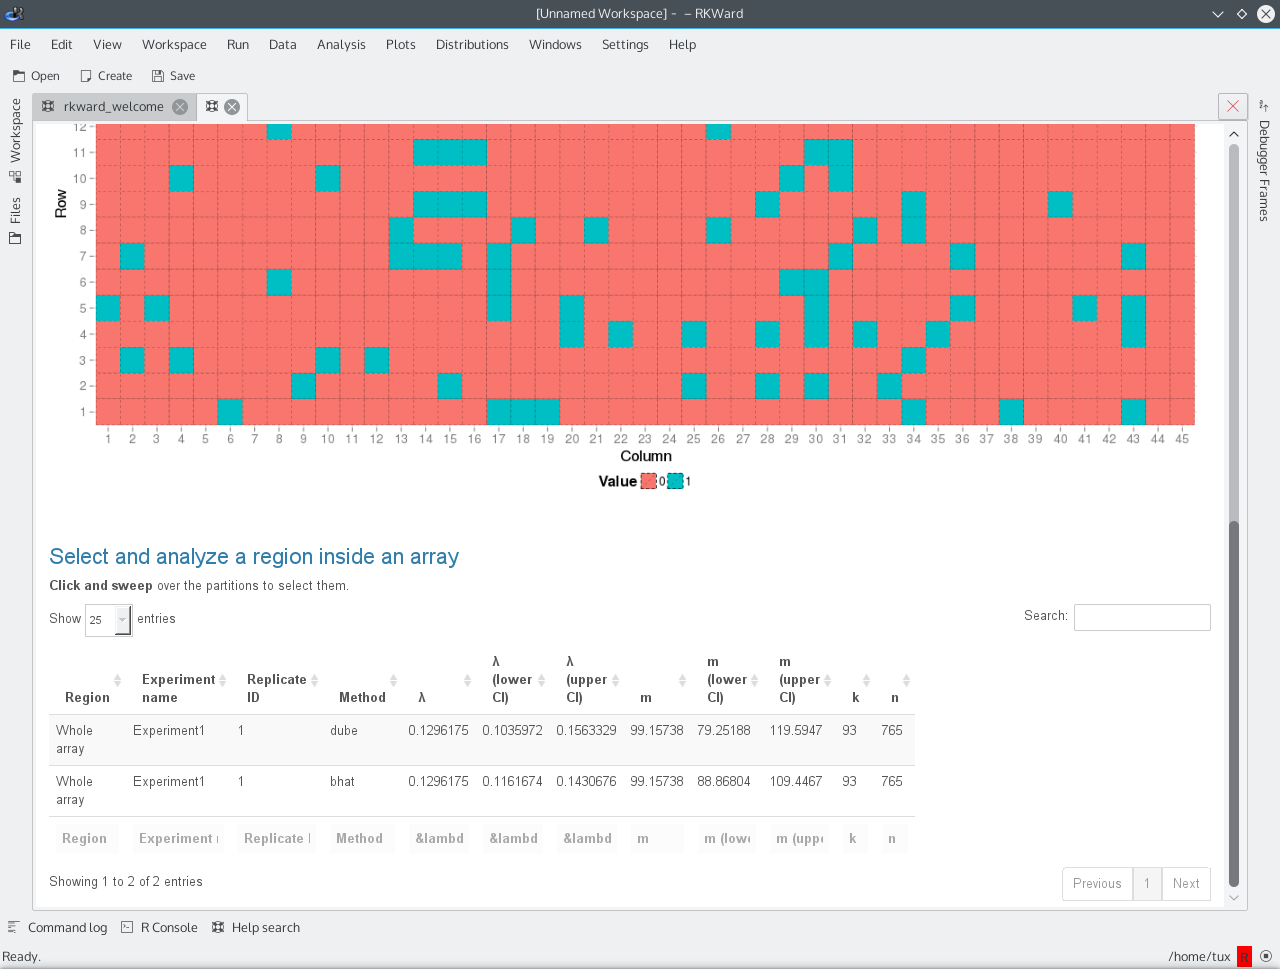
\includegraphics[width=17cm]{GUI_RKWard_1.png}
\end{center}
\caption{\textit{dpcrReport()} function running in the graphical user interface and integrated development environment \textbf{RKWard}.}
\label{GUI_RKWard_1}
\end{figure*}

\subsection{Materials subsection Statistical power - Monte Carlo simulations}

The proposed framework was evaluated in three Monte Carlo experiments (2.000 times repetitions each) with accordingly 1.000, 5.000 (results not shown) and 10.000 partitions. During each repetition of the Monte Carlo scheme, a set of partitions was randomly generated~\cite{dube_mathematical_2008} with a determined number of molecules ('Base number of molecules' on X-axis). The set was copied and a number of molecules ('Added number of molecules' on Y-axis) was added to randomly chosen partitions. Two obtained arrays were compared using the proposed method. The mean p-values alongside with their standard deviation are presented in the chart below.

\begin{figure}[t]
\begin{center}
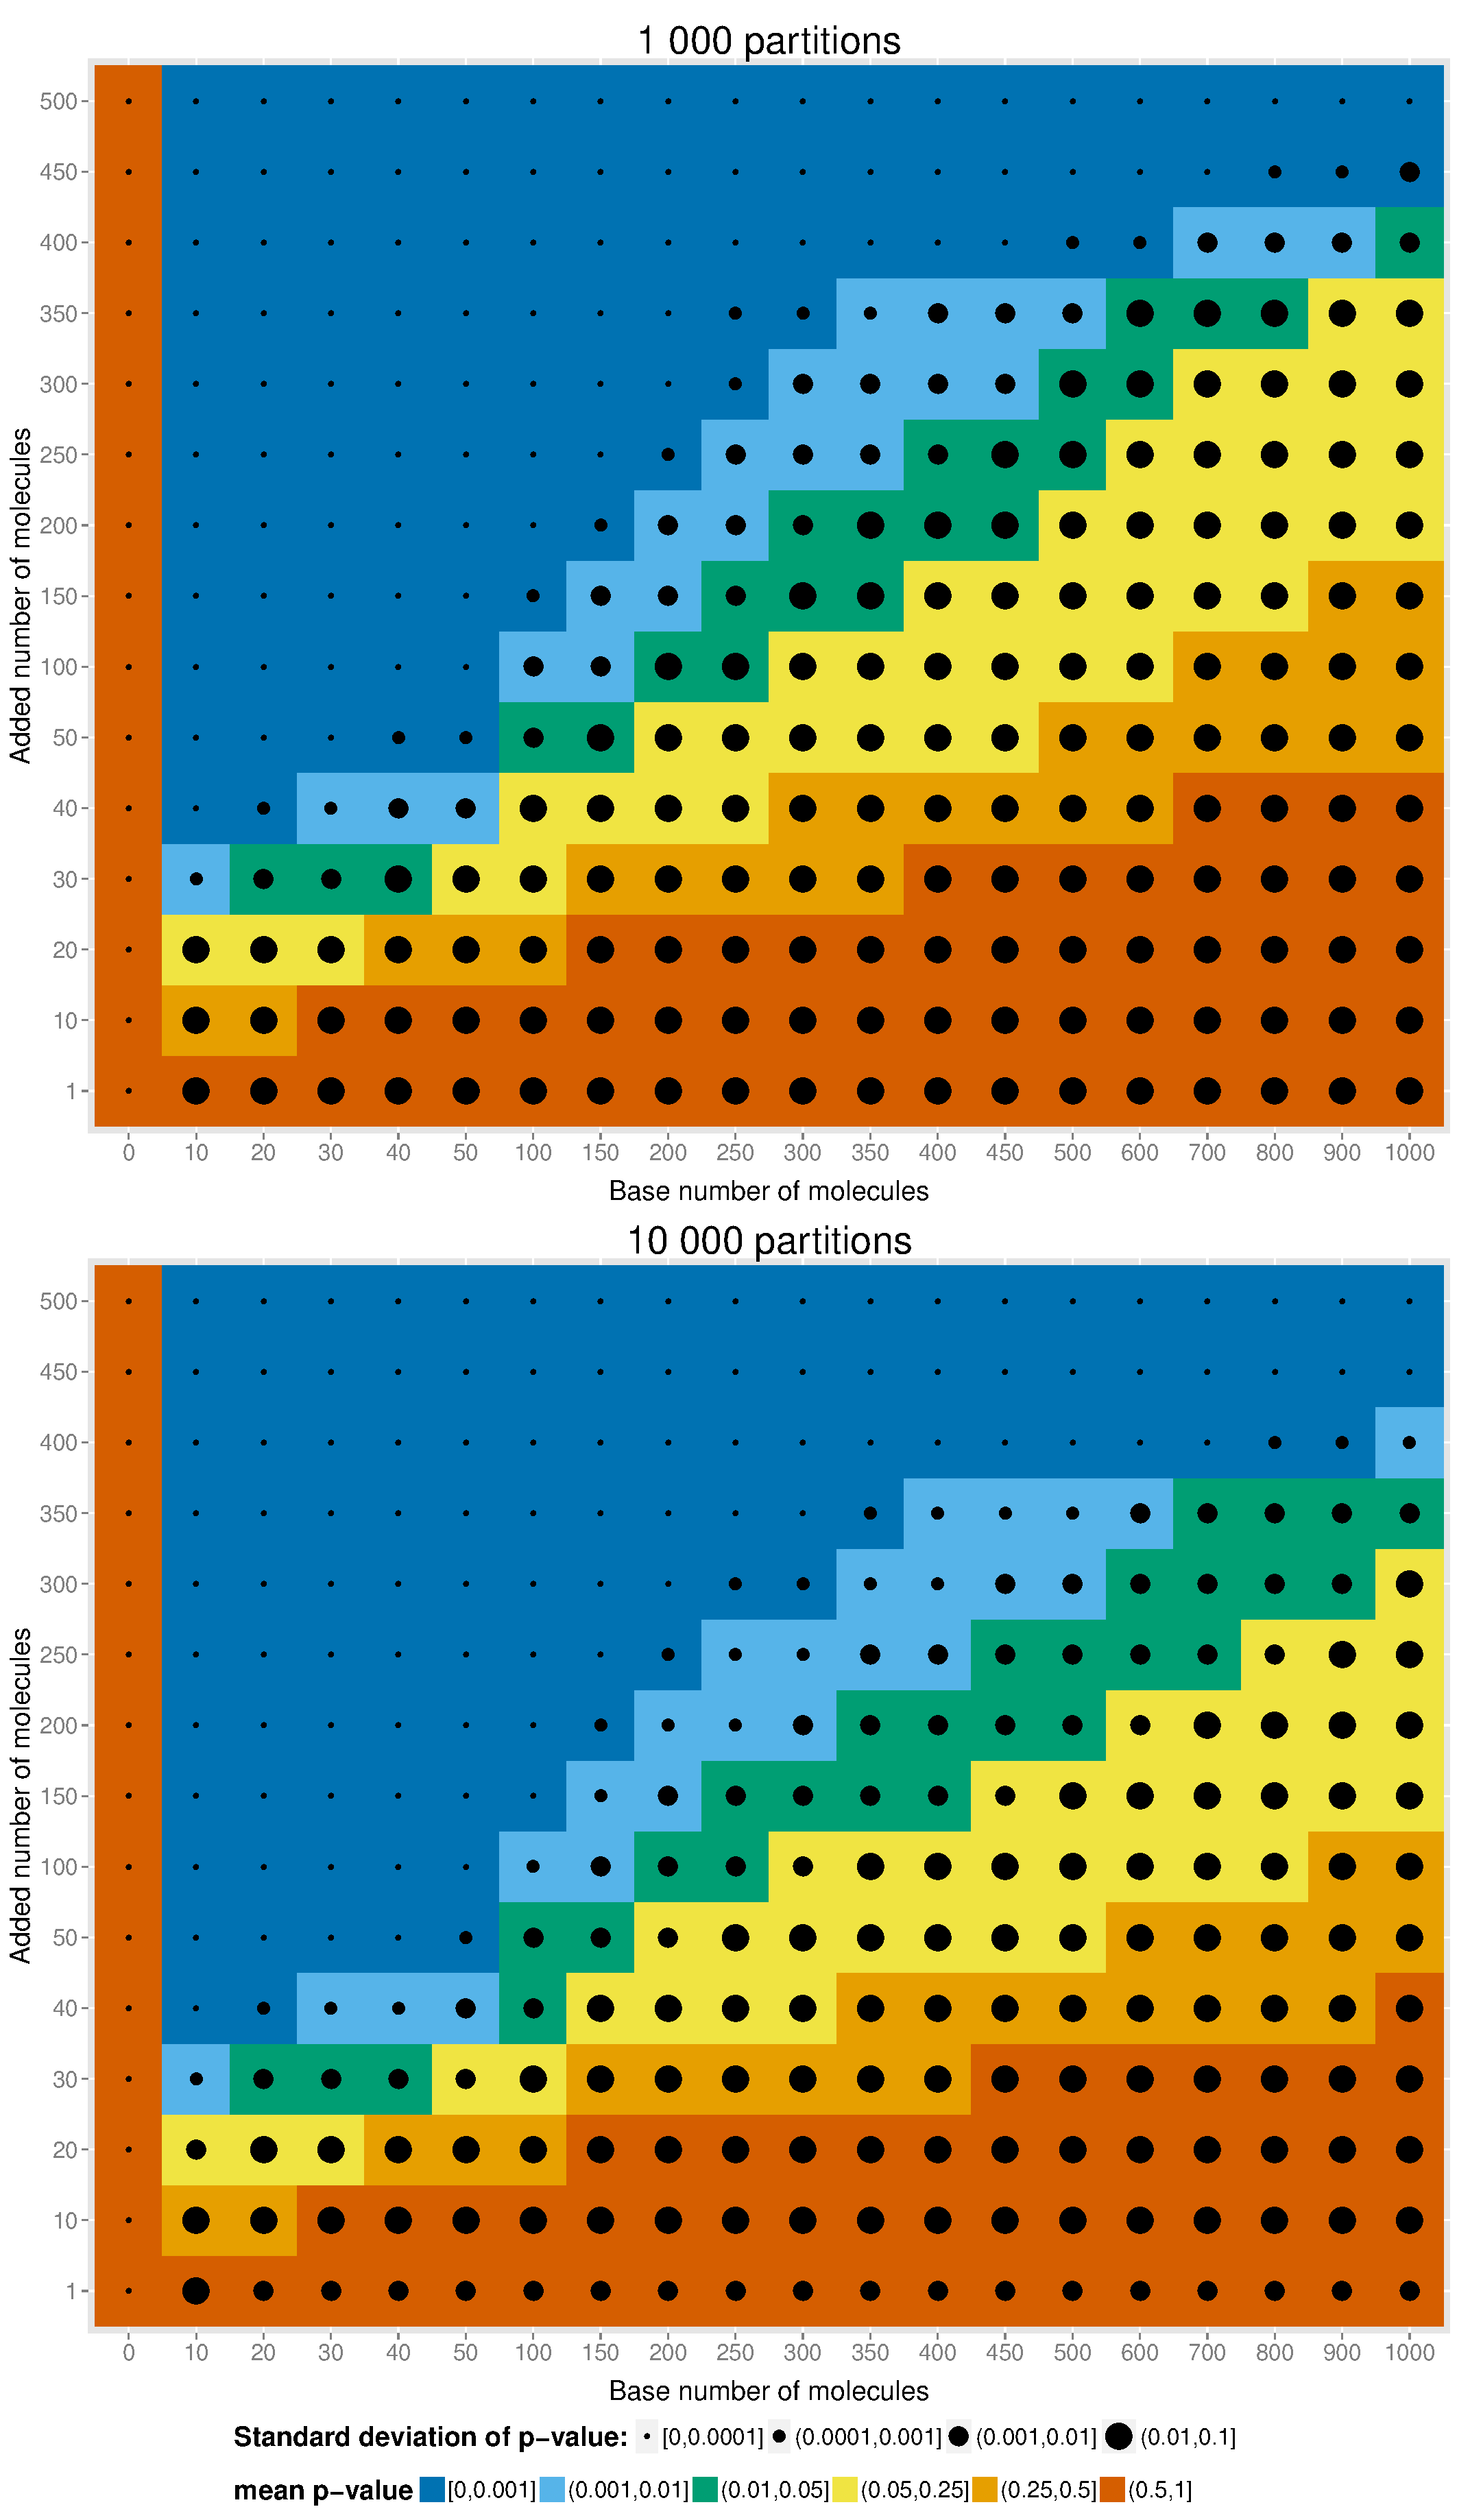
\includegraphics[width=9cm]{mc_figures-1.pdf}
\end{center}
\caption{Our method, based on GLM, predicts estimated means copies per partitions using Poisson or binomial regression. Afterwards, estimates are compared against themselves using t-test. Obtained p-values and confidence intervals do not require further correction, because the familywise error is controlled through the whole analysis.}
\label{mc_figures-1}
\end{figure}

\subsection{Import and export of results figures and data}.

\subsubsection{Reading or importing data}

\textbf{R} has a rich set of tool to arrange data (reshape \cite{Wickham_2007}) 
in order to prepare them for the analysis. This is important when it comes to 
the question how experiments should be treated.

Most \textit{dpcR} import functions take a data matrix of annotated numeric 
(e.g, fluorescence amplitude) and integer values (e.g., counts) as input. The 
\textit{raw\_data} input was implemented  make data input easier for the end 
user (see Supplement). Such input files can be manually created in a spreadsheet 
program or text editor.

(see Table \ref{table_formats}).

\begin{table}[b]
\tableparts{%
\caption{Structured vendor export data formats handled by \textit{dpcR}~v.~0.5 and later.}
\label{table_formats}%
}{%
\begin{tabular*}{\columnwidth}{@{}llll@{}}
\toprule
Vendor & System & Format & Type
\\
\colrule
Bio-Rad & QX100 \& QX200 & CSV & Summary export
\\
Fluidigm & BioMark & CSV & Summary export
\\
Formulatrix & Constellation Digital PCR & CSV & Summary export
\\
\botrule
\end{tabular*}%
} {The number of structured export data formats handled by \textit{dpcR} is 
growing. Numerous data formats can be processed with the functionality provided 
by the \textbf{R} environment (see \cite{rodiger_r_2015}). CSV, comma separated 
values.}
\end{table}

\subsubsection{\textit{De novo} creation of dpcR objects from raw data}

In experimental setups user have the need to transform their raw data in a 
processable format. Since the \textbf{R} environment is cross-platform an 
ubiquitously used we aimed to ease this creation. In particular, this is 
relevant for reproducible research. The \textit{dpcR} framework covers the types 
typically used in laboratories.

\subsubsection{Public data sets}

\textit{dpcR} includes data sets or refers to additional R packages for testing 
purposes. The data originate from different dPCR and qPCR systems and were 
either published previously \cite{whale_comparison_2012, roediger2015chippcr, 
white_digital_2009, rodiger_r_2015} or \textit{de novo} generated.

\subsubsection{Export of analysis results}

Since \textit{dpcR} is based on the \textbf{R} environment all facilities for a 
report generation are usable as described before \cite{rodiger_r_2015}.

(see Table \ref{table_formats}).

A commonly available data exchange format is a perquisite for reproducible 
research. So far no cross-platform and system-independent format has been 
introduced for dPCR experiments. Therefore, we decided to use \texttt{RData} as 
our default format. \texttt{RData} works across all \textbf{R} environments and 
saves the variable names along the content of multiple variables, which can be 
restored in any workspace.


\subsection{Calculation of the ``Concentration''}
Reference to ``Supplement''

qPCR	dPCR
Number of copies/DNA per volume (e.g., ng/µl, copies/µl)	total number of compartments * ln (...)

Two-sided exact tests and matching confidence intervals for discrete data \cite{fay_2010}

Controlling the False Discovery Rate: A Practical and Powerful Approach to Multiple Testing \cite{benjamini_1995}

Interval Estimation for a Binomial Proportion \cite{brown_2001}

\subsection{Converting qPCRs to dPCRs}

qPCR is a well established and robust technology, which allows precise 
quantification of DNA material in high throughput fashion. Such systems can be 
used for dPCR applications. The real-time monitoring of the PCR product 
formation enables to determine quantification points (Cq). The Cq are strictly 
related to the input quantity. A simple arithmetic operation (after logarithmic 
transformation of the concentration) is sufficient to determine any nucleic acid 
quantity \cite{huggett_considerations_2014}. The quantification of the 
amplification is not done by determining a Cq value derived from an 
amplification curve. However, the quantification by qPCR is challenging at very 
low and very high concentrations. At low DNA concentration Monte Carlo effect 
play a role and at high concentration inhibition processes start to dominate the 
qPCR. Thus, the qPCR is only usable in the working range of the calibrator. In 
addition, pre-processing and data analysis is a affected by numerous adverse 
effects \cite{ruijter_2013, pabinger_survey_2014, spiess_impact_2015}.

Figure\ref{qpcr2pp_1}

\begin{figure}[t]
\begin{center}
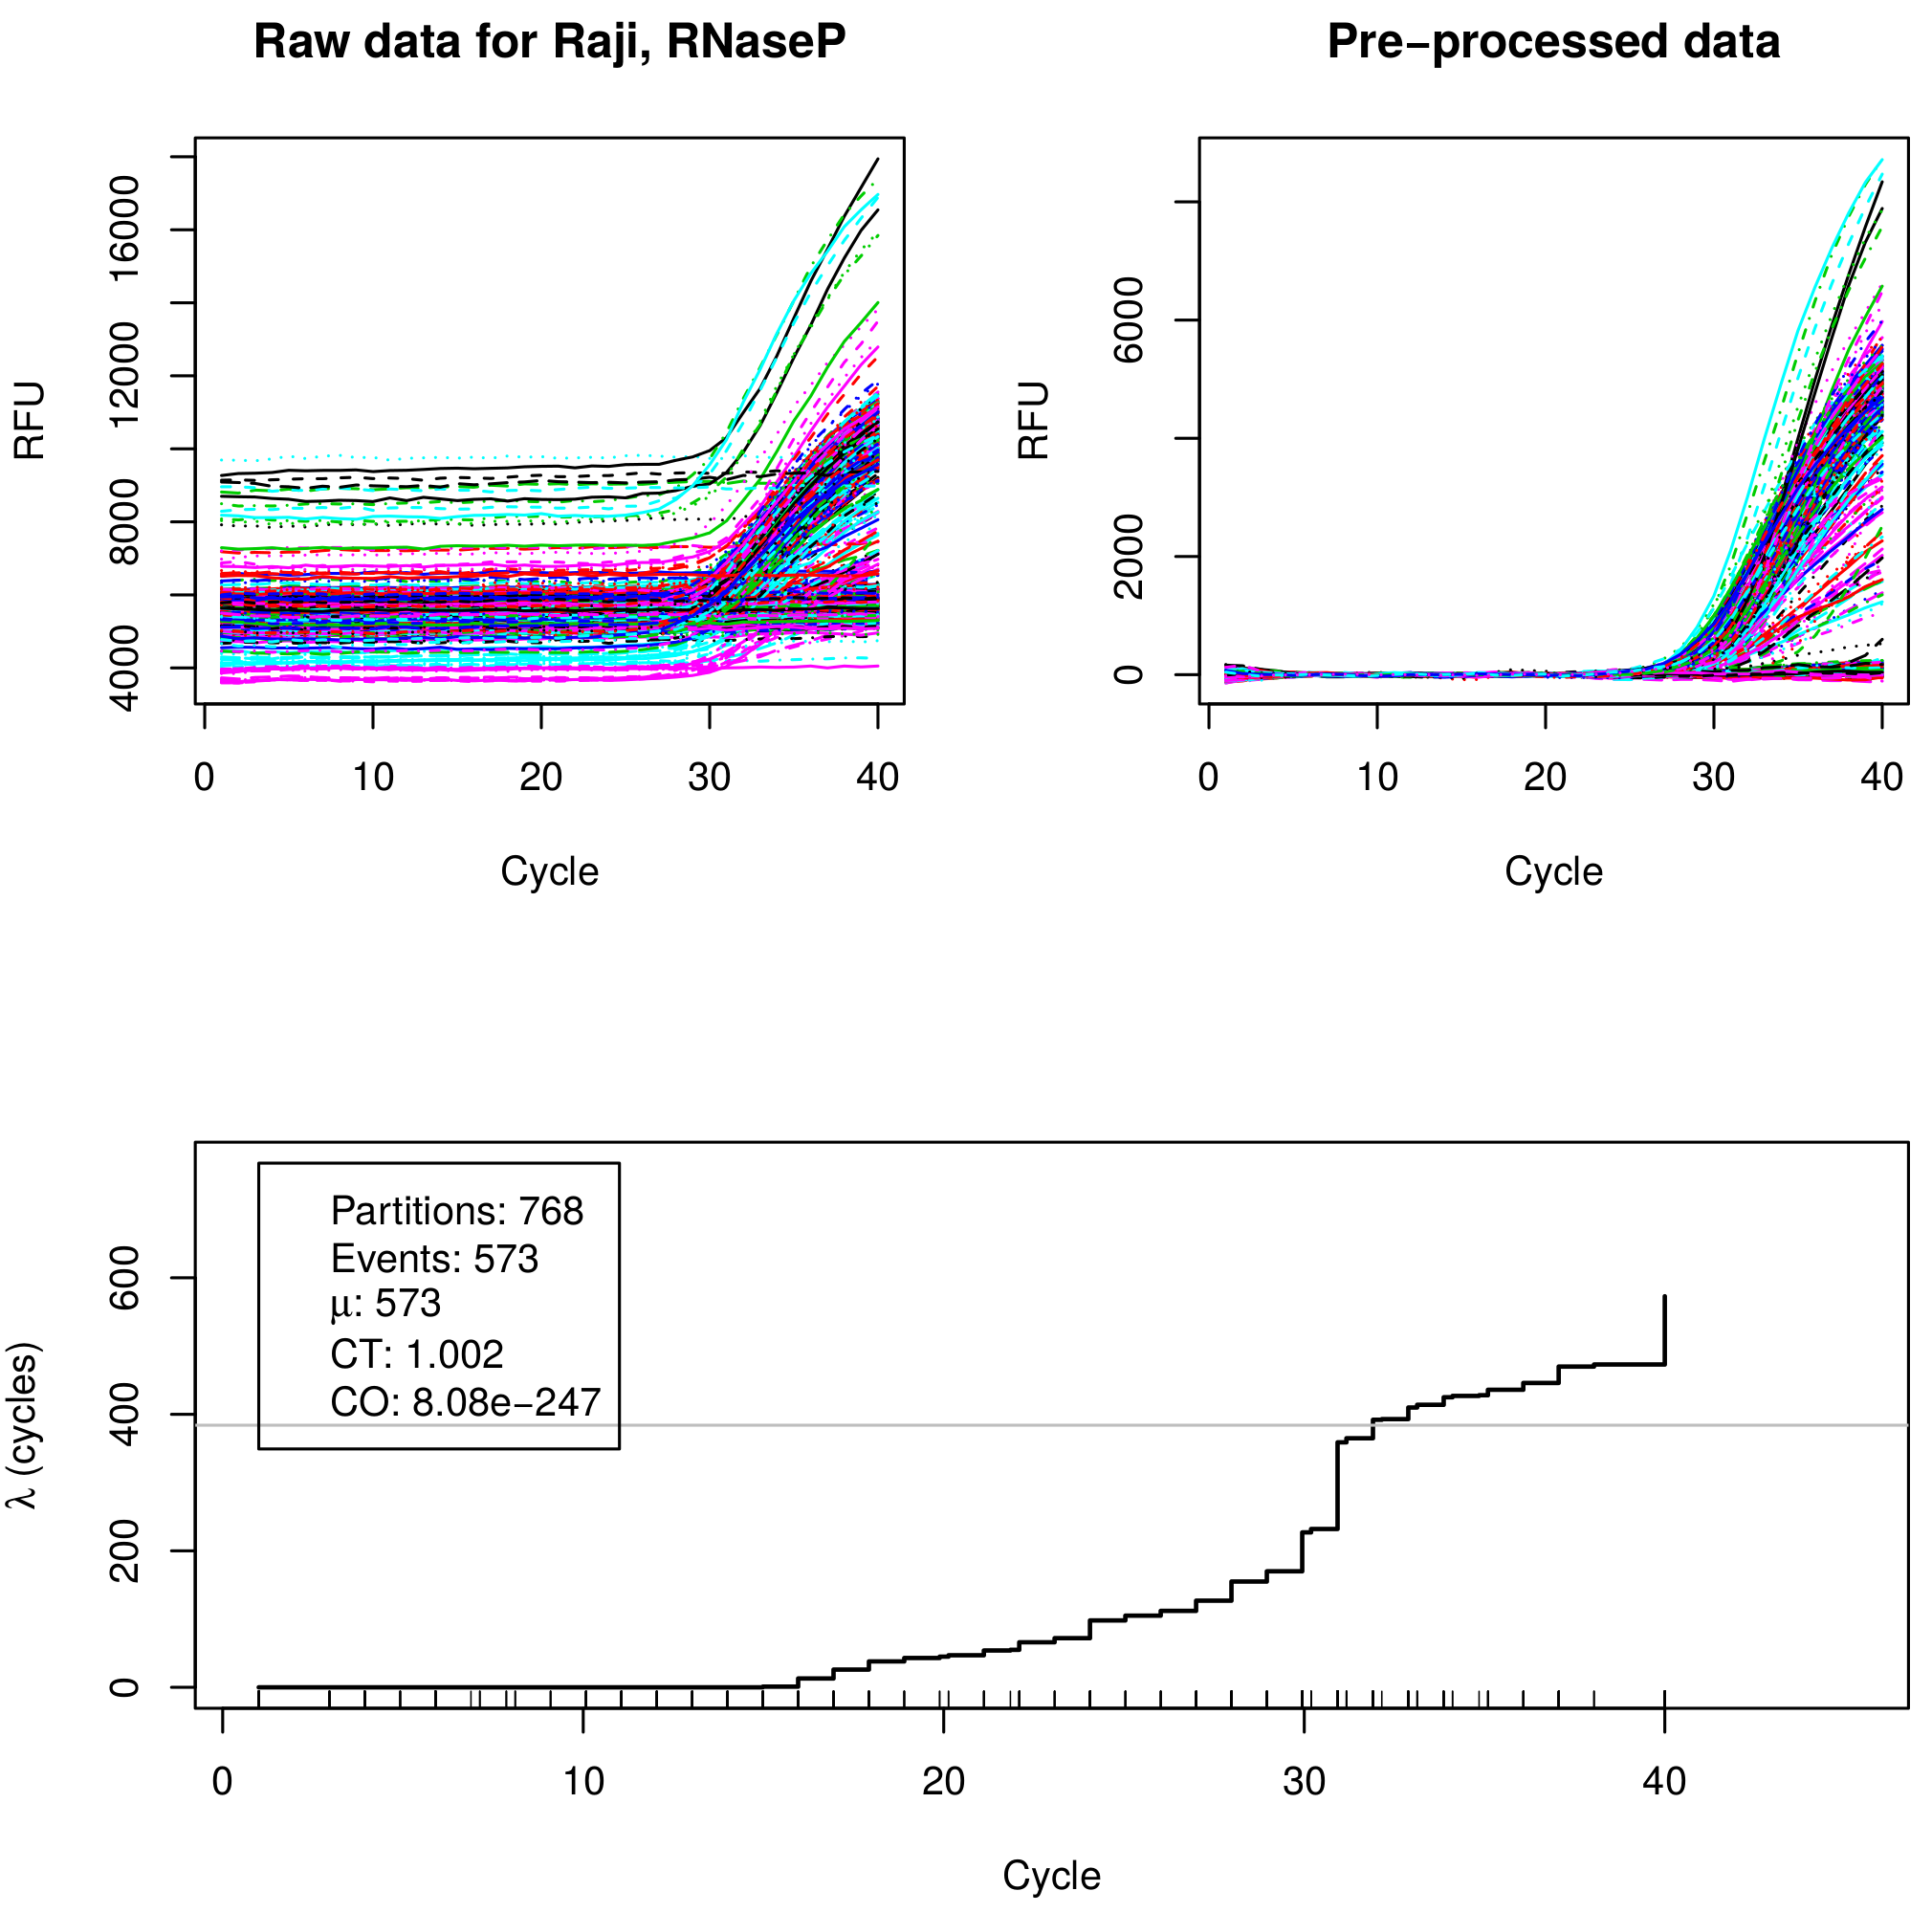
\includegraphics[width=9cm]{qpcr2pp_1.png}
\end{center}
\caption{Uncover characteristics of dPCR data. 
Selected dPCR platforms are qPCR platforms at the same time. The function \textit{qpcr2pp} uses the 
qPCR amplification curve data and interprets them as dPCR (Poisson process). A) Raw data of The 
function were B) preprocessed (baselined, smoothed) with functions from the 
\textit{chipPCR} package and C) finally analyzed (Cq calculation $\rightarrow$ binarize) with the 
\textit{qpcr2pp} (qPCR to Poisson process) function from the \textit{dpcR} package.} 
\label{qpcr2pp_1}
\end{figure}

As described in \cite{ritz_qpcr_2008, perkins_readqpcr_2012, 
pabinger_survey_2014, rodiger_r_2015}, there numerous methods to import 
amplification curve data into the \textbf{R} workspace. Prior processing the 
data for dPCR analysis it is recommended to use dedicated \textbf{R} packages, 
such as \textit{chipPCR} \cite{roediger2015chippcr}, \textit{MBmca} 
\cite{rodiger_surface_2013}, \textit{qpcR} \cite{ritz_qpcr_2008}, to 
pre-process (e.g., removal of missing values, smoothing 
\cite{spiess_impact_2015}) the raw data.

\section{RESULTS}

In the following section we show two case studies for the use of the \textit{dpcR} package.

\subsection{Availability}

The \textit{dpcR} framework is available as open source software package (GPL-3 
or later) as part of the Bioconductor project \cite{gentleman_2004}. The stable 
version is hosted at http://cran.r-project.org/web/packages/dpcR and the source 
code is available from  https://github.com/michbur/dpcR.

\section{DISCUSSION}

Currently, there exist different dPCR analysis software solutions provided by 
the vendors. But most of the software packages are designed black boxes, which 
prevent deep insight into the data processing step. Other and we think that 
scientific software should be open \cite{morin_shining_2012, ince_case_2012, 
rodiger_r_2015}. In addition, most of the software solutions are aimed to be 
used in very specific scenarios and a mutual exclusive to alternative platforms 
(e.g., droplet vs. chamber-based). We have chosen \textbf{R} because it is the 
\textit{lingua franca} in biostatistics and broadly used in other disciplines 
\cite{rodiger_r_2015}. We developed the \textit{dpcR} package, which is a 
software framework for analysis of dPCR. \textit{dpcR} provides the scientific 
community a broadly applicable tool for teaching purposes, data analysis and 
theoretical research based on simulations. Our software framework can be used to 
accelerate the development of new approaches to dPCR.

In \cite{rodiger_r_2015} we gave an example where we re-analyze droplet dPCR 
data from a Bio-Rad QX100 system with an early implementation of the 
\textit{dpcR} package.

We implemented numerous statistical methods for dPCR and suggest the 
introduction of a standardized nomenclature for dPCR. The package enables the 
simulations and predictions of dPCR reactions and the analysis of previously run dPCRs.

Functions included may be used to simulate dPCRs, perform statistical data 
analysis, plotting of the results and simple report generation. 

We decided not to implement algorithms for clustering and ``rain'' (positive droplets) definition of 
droplet dPCR data. This is because, there are several \textbf{R} packages from 
flow-cytometer research. Implementations range from manual to automatic 
clustering \cite{le_meur_computational_2013, Malek15022015, trypsteen_ddpcrquant_2015}. Moreover, 
discussion with our peers and the literature suggest that a consensus of an 
appropriate method for dPCR is not available.

\section{CONCLUSION}

In conclusion, \textit{dpcR} provides means to understand how digital PCR works, 
to design, simulate and analyze experiments, and to verify their results (e.g., 
confidence interval estimation), which should ultimately improve 
reproducibility. We have built what we believe to be the first unified, 
cross-platform, dMIQE compliant, open source software framework for 
analyzing dPCR experiments. Our \textit{dpcR} framework is 
targeted at a broad user base including end users in clinics, academics, 
developers, and educators. We implemented existing statistical methods for dPCR 
and suggest the introduction of a standardized dPCR nomenclature. Our 
framework is suitable for teaching and includes references for an elaborated 
set of methods for dPCR statistics. Our software can be used for (I) data 
analysis and visualization in research, (II) as software framework for novel 
technical developments, (III) as platform for teaching this new technology and 
(IV) as reference for statistical methods with a standardized nomenclature for 
dPCR experiments. The framework enables the simulations and predictions of Poisson 
distribution for dPCR scenarios, the analysis of previously run dPCRs. Due to 
the plug-in structure of the software it is possible to build custom-made 
analyzers.

Our open framework includes to invitation to the scientific community to join and 
support the development of \textit{dpcR}.


\section{ACKNOWLEDGEMENTS}

Grateful thanks belong to the \textbf{R} community and the \textbf{RStudio} developers.

\section{Funding}
This work was funded by the Federal Ministry of Education and Research (BMBF) InnoProfile--Transfer--Projekt 03 IPT 611X.
 
\subsubsection{Conflict of interest statement.} None declared.
%\newpage

\bibliographystyle{plain}
\bibliography{dpcr}
\end{document}
